
\documentclass[conference]{IEEEtran}
\IEEEoverridecommandlockouts
% The preceding line is only needed to identify funding in the first footnote. If that is unneeded, please comment it out.
\usepackage{cite}
\usepackage{amsmath,amssymb,amsfonts}
\usepackage{graphicx}
\usepackage{textcomp}
\usepackage{xcolor}
\usepackage{hyperref}
\usepackage{etoolbox}

\def\BibTeX{{\rm B\kern-.05em{\sc i\kern-.025em b}\kern-.08em
    T\kern-.1667em\lower.7ex\hbox{E}\kern-.125emX}} 

\begin{document}

\title{\textbf{World Development Analysis Application}\\
\vspace{10pt}
\Large Information Visualization, University of Aveiro \\ 2019
}

\author{\IEEEauthorblockN{Filipe Pires, 85122}
\IEEEauthorblockA{\textit{DETI, MSc. Informatics Engineering}}
\and
\IEEEauthorblockN{João Alegria, 85048}
\IEEEauthorblockA{\textit{DETI, MSc. Informatics Engineering}}

}

\makeatletter
\patchcmd{\@maketitle}
{\addvspace{0.5\baselineskip}\egroup}
{\addvspace{-1\baselineskip}\egroup}
{}
{}
\makeatother

\maketitle

\begin{abstract}
The use of graphical tools for information visualization has become an intrinsic 
part of our daily lives.
Whether it is the structure of a text messages app or a dashboard to monitor a 
power plant, man kind is not only used to, but very much specialized 
at interpreting data through sight. 

This has led to a great development of the field, with numerous tools being
developed constantly and helpful technologies being spread throughout creators.

In this report we explore a well known web development tool called D3.js and 
present some of its potential through the use case of a World Development 
Indicators analysis.
\end{abstract} 

% \begin{IEEEkeywords}
% data visualization, ...
% \end{IEEEkeywords}

\section{Introduction}

As visually treating information settles permanently in our lives, many tasks 
have their complexities reduced by adopting graphical tools.
Also, with the recent boom of data flowing through the internet and our devices, 
a need for tools to be more robust, faster and more hardware agnostic emerges 
in the visualization information community.

D3.js appears as a JavaScript library for manipulating documents \cite{d3}, with 
potential to answer many market requirements.
By focusing on web standards, D3 gives creators the full capabilities of modern 
browsers, combining powerful visualization components and a data-driven approach 
to DOM manipulation. 

This report is the result of a proposal made for the course of Information
Visualization \cite{proj} and describes the work aimed to explore the 
capabilities of D3 for visualizing data in a intuitive way.
Our work follows a case study, focused on providing a website of 
analysis of world development indicators.

All of the written code is available at our  
\href{https://github.com/joao-alegria/VI}{GitHub repository}, following professor Tiago Davi's
\href{https://github.com/tiagodavi70/ua_infovis/blob/c50422815f49b0a4747c6f727042b4da95dd7af2/D3/Code_Style.md}{Code Style Guide}.
We also provide access to a video demonstration of the website, along with 
the necessary instructions on how to test the code.

\section{Dataset}

The information source was taken from the World Bank, through Kaggle \cite{kaggle}.
It is a data base containing over a thousand annual world development indicators
from hundreds of countries.
We focus on a specific set of indicators somehow related in order to maintain 
coherence throughout the website and to scale the data to the level of complexity 
demanded.

After studying the indicators, we selected those about death rates and related 
health indicators.
The chosen fields were: mortality rate attributed to unsafe water and sanitation,
and lack of hygiene; suicide mortality rate; mortality rate, neonatal, under-5, 
infant and adult; incidence of malaria, HIV, tuberculosis; intentional 
homicides; number of nurses and midwives.

Through a Python script, we collected the columns from the downloaded dataset in 
CSV format.
Then, we applied a transformation so that all were in the same unit of measure.
As all indicators referred to an amount of people per either $10^3$ or $10^5$ 
people, we converted them to the scale of X per 100 000 people, where X is the 
value of each field. This normalized the data and made comparisons more intuitive.
The script also stored the relevant fields in a JSON format for ease of access.

\section{Users and the Questions}

But before writting any line of code, we came to an agreement on who would the 
target audience be and what visualization tools would be more appropriate for them.

% \subsection{Characterization of the Users and their Context}

As the data could be useful both in specific research environments and in more
general cases of information searching, we decided to define the target audience
as casual users seeking to gain general knowledge about our development indicators.
The unit of measure used and the nature of the development indicators made it
easier for any user with no specialized background knowledge to be able to learn
from the tools we intended to develop, so we proceeded with this approach.

% \subsection{Questions to be Answered}

Nevertheless, some guidelines had to be defined regarding what exactly would
the website be able to deliver and what kind of answers could the visitors find in it.
With this in mind, we established 3 major questions for the solution:
\begin{itemize}
    \item How are countries related regarding death rates?
    \item How does a country's indicator evolve over time?
    \item What indicators may affect number of deaths?
\end{itemize}

\section{Visualization Solution}

The development phase had two major periods: 
brainstorming, planning, prototyping and receiving feedback;
implementing a functional prototype with the use of the D3.js library.

\subsection{Low Fidelity Prototype and User Feedback}

Based on the questions previously stated, we created a paper prototype that 
served as a sketch of the website and drew the graphical elements in it.
Then, we simulated the use of the website with a few colleagues and removed 
distracting elements and unnecessary details.

We also presented the prototype to more experienced users, professionals of the
field of information visualization, in order to avoid bringing design errors to
the next phase of development.
The result was the removal of the concept of tabs and the structuring of the 
website in a single page with transitions between tabs based on scrolling.

\subsection{Functional Prototype}

The prototype's first tool is a world map with color codification.
Our choice was based on the knowledge that map visualizations offer the most 
natural way of presenting geographically-dependent data, and encoding our 
dataset with the right colors makes possible countries comparisons.

\begin{figure}[h!]
\centering
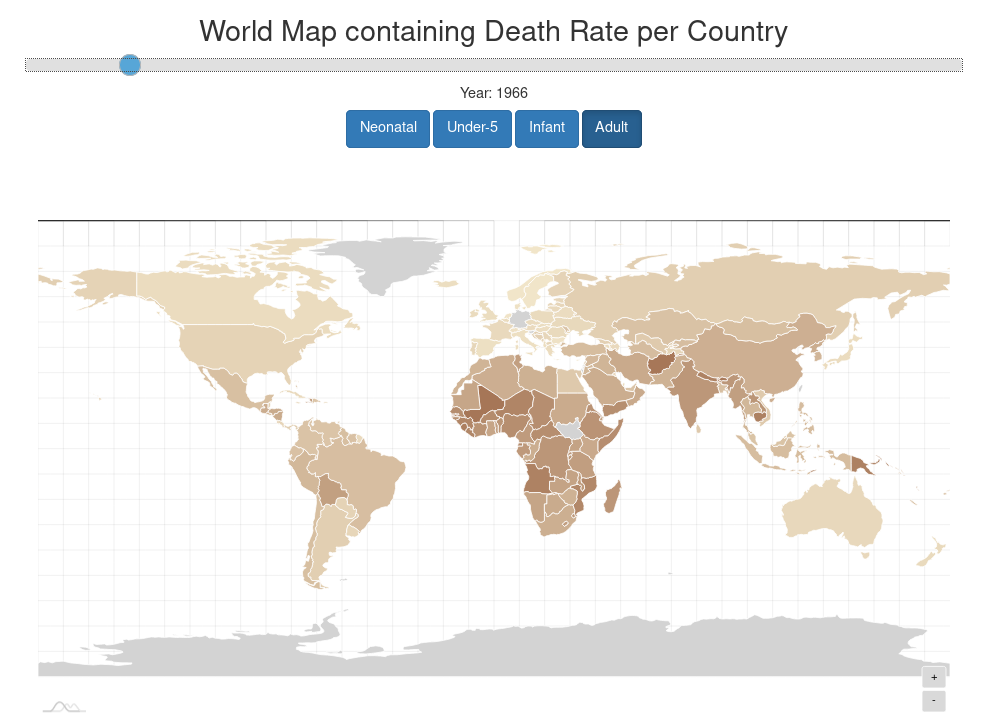
\includegraphics[width=0.95\linewidth]{../img/screenshots/screenshot_map.png}
\caption{Screen capture of our prototype's world map.}
\label{fig:worldmap}
\end{figure}

The map, visible in Fig. \ref{fig:worldmap}, presents the death rate indicator of one 
age range at a time and the user can select which age range to analyse.
The data is restricted to one year.
However, as the dataset's time range is large enough, we came up with the 
solution of a wide slider - this gave us the advantage of giving the user an 
appealing, although partial, notion of the answer to the second question by 
slowly moving the slider from left to right and keeping track of the evolution 
worldwide.

With the help of Coblis \cite{coblis}, a color blindness simulator, we were able 
to select a color palette for the map that worked for all types of color vision 
deficiencies (except monochromacy, as the countries without data are encoded in grey).

\begin{figure}[h!]
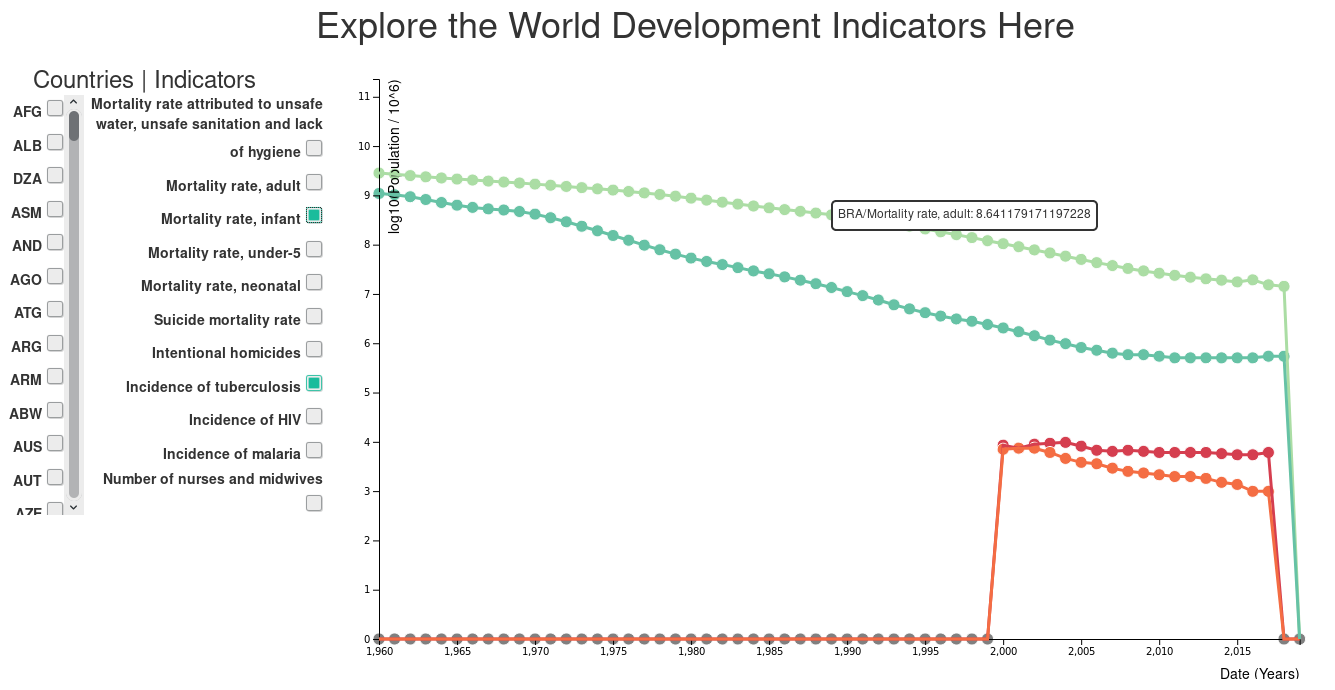
\includegraphics[width=\linewidth]{../img/screenshots/screenshot_connectedscatterplot.png}
\caption{Screen capture of our prototype's connected scatter-plot.}
\label{fig:scatterplot}
\end{figure}

The connected scatter-plot, seen in Fig. \ref{fig:scatterplot} was our second 
developed tool, and it complements the first one in many ways.
By presenting time in the x axis and the values of each indicator in the y axis,
not only is the user able to track time evolution with high precision, but he/she
can now compare them and search for patterns or correlations.
But what is even more empowering is the ability to compare 1 or more indicators
between several countries simultaneously.
All indicators become available here, and when the user clicks a country on the 
map he/she is automatically directed to the scatter plot with the country 
selected and the death rate active.

We use color codification simply to distinguish lines and add useful 
tooltips to the connected points.
Brushing is also available to define what range of years interests the user.
Empty entries are attributed the value of zero in the plot.

Note: the world map also contains tooltips and a color range label connected to 
them to guide the user and for greater detail.

\subsection{Implementation Challenges}

The brushing feature was probably the most effort demanding task during development,
but there were actually no significant problems worth mentioning.
The graphical components were built with the help of AMCharts \cite{amcharts}, a
JavaScript library that uses D3.js, providing us with the basis of our tools.

\subsection{Evaluation and Changes to the Prototype}

Once a stable version of the website was completed, we proceeded to evaluating 
its usability through a cognitive walkthrough.
The procedure was done with 6 users and they were proposed to answer 5 questions 
using the website's tools.

We added a small introduction on the home page to guide visitors and a 
description of the work at the bottom.
Participants had no trouble understanding how to navigate around.
However, users had some difficulties in selecting several countries for the 
scatter plot and found that setting unknown values as zero was deceiving.
One small detail mentioned by 1 participant was that indicators didn't follow 
a logical order.

We then corrected the solution by ordering the indicators and making unknown 
values as grey points.
We also added the ability to select more than 1 country on the map.

\section{Conclusion and Future Work}

By the end of this project, it became clear to us why D3 became so popular; 
its ease of use, flexibility and wide range of controls makes it a very appealing 
library for any scenario of data visualization.
We also take from this project a better mindset for developing visual data 
analysis tools, as it gave us the chance to apply not only what we studied but 
also aspects we had to learn along the way.

Although we do not go much into detail in the evaluation tests, we found these
extremely useful and were able to substantially improve the solution's quality
through them.
For future work, the next steps would be to add a search tab on the countries 
filter for a faster selection, and optimize the map slider to make its use 
smoother.


% \begin{itemize}
% \item Lorem ipsum ...
% \end{itemize}

% \begin{equation}
% a+b=\gamma\label{eq}
% \end{equation}

% ... \eqref{eq} ...

% ... Fig.~\ref{fig} ...

% \begin{table}[htbp]
% \caption{Table Type Styles}
% \begin{center}
% \begin{tabular}{|c|c|c|c|}
% \hline
% \textbf{Table}&\multicolumn{3}{|c|}{\textbf{Table Column Head}} \\
% \cline{2-4} 
% \textbf{Head} & \textbf{\textit{Table column subhead}}& \textbf{\textit{Subhead}}& \textbf{\textit{Subhead}} \\
% \hline
% copy& More table copy$^{\mathrm{a}}$& &  \\
% \hline
% \multicolumn{4}{l}{$^{\mathrm{a}}$Sample of a Table footnote.}
% \end{tabular}
% \label{tab1}
% \end{center}
% \end{table}

% \begin{figure}[htbp]
% \centerline{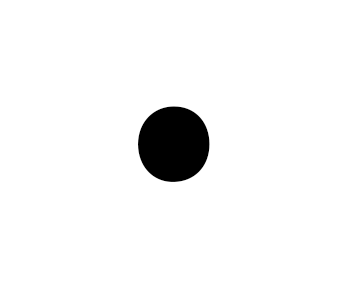
\includegraphics{fig1.png}}
% \caption{Example of a figure caption.}
% \label{fig}
% \end{figure}

\begin{thebibliography}{00}
\bibitem{d3} M. Bostock, "D3", \url{https://d3js.org/}, accessed in November 2019.
\bibitem{proj} B. S. Santos, T. Davi, "Diretivas para o Trabalho de Design", DETI, University of Aveiro, November 2019.
\bibitem{kaggle} World Bank, "World Development Indicators", \url{https://www.kaggle.com/worldbank/world-development-indicators}, accessed in November 2019.
\bibitem{coblis} Colblindor, "Coblis - Color Blindness Simulator", \url{https://www.color-blindness.com/coblis-color-blindness-simulator/}, accessed in November 2019.
\bibitem{amcharts} amCharts, "JavaScript Charts \& Maps", \url{https://www.amcharts.com/}, accessed in November 2019.
\end{thebibliography}
\vspace{12pt}



\end{document}
